% m und b für lin Reg Blau: [-4.369633789234495e-05+/-2.9709254353727494e-06
%  4.778847991795171e-05+/-2.6717001118211153e-06]
% Grenspannung Blau: U_G= 1.09+/-0.10V
%  mit x=(y-b)/m
% m und b für lin Reg Grün: [-1.5606083440180905e-05+/-1.3253599150127752e-06
%  9.669029888654872e-06+/-6.558411515946087e-07]
% Grenspannung Grün: U_G= 0.62+/-0.07V
% m und b für lin Reg Orange: [-1.2179617482918451e-05+/-7.693172875330904e-07
%  6.522199692258643e-06+/-3.2820197170611725e-07]
% Grenspannung Orange: U_G= 0.54+/-0.04V
% m und b für lin Reg Violet: [-7.012170046339161e-06+/-6.994029084373119e-07
%  8.505155840994801e-06+/-6.675543373720807e-07]
% Grenspannung Violet: U_G= 1.21+/-0.15V
% m und b von f-U Diagramm berechnet [3.218938942773891e-15+/-9.772583238801467e-17
%  -1.139712862517234+/-0.06151769246689413]
% m und b von f-U Diagramm gemessen [2.7780757270797524e-15+/-2.373012528761886e-16
%  -0.9080012215304237+/-0.14937939151648477]
% e = 1.602176634e-19
% h = 4.135667696923859e-15
\nocite{anleitungV500}
\section{Auswertung}
\label{sec:Auswertung}
\begin{table}[H]
    \centering
    \caption{Gemesse Stromstärke in Abhängigkeit der Spannung.}
    \label{tab:Strom-Spannung}
    \begin{tblr}{colspec ={c c || c c || c c}}
        \toprule
        $U\,[\unit{\volt}]$ & $I\,[\unit{\nano\ampere}]$ & $U\,[\unit{\volt}]$ & $I\,[\unit{\nano\ampere}]$ & $U\,[\unit{\volt}]$ & $I\,[\unit{\nano\ampere}]$\\
        \midrule
        -1,05   & 0     & -0,80   & 0,160 & -0,02   & 1,350\\
        -1,00   & 0,030 & -0,78   & 0,175 & 1,00    & 2,600\\
        -0,96   & 0,038 & -0,76   & 0,200 & 3,00    & 5,800\\
        -0,94   & 0,052 & -0,74   & 0,230 & 6,00    & 9,200\\
        -0,92   & 0,062 & -0,72   & 0,255 & 9,00    & 11,00\\
        -0,90   & 0,078 & -0,70   & 0,280 & 12,00   & 12,50\\
        -0,88   & 0,090 & -0,65   & 0,360 & 15,00   & 14,00\\
        -0,86   & 0,105 & -0,60   & 0,440 & 18,00   & 15,00\\
        -0,84   & 0,115 & -0,55   & 0,520 & 19,00   & 15,00\\
        -0,82   & 0,140 & -0,50   & 0,600 &  & \\
        \bottomrule
    \end{tblr}
\end{table}
% \begin{figure}
%   \centering
%   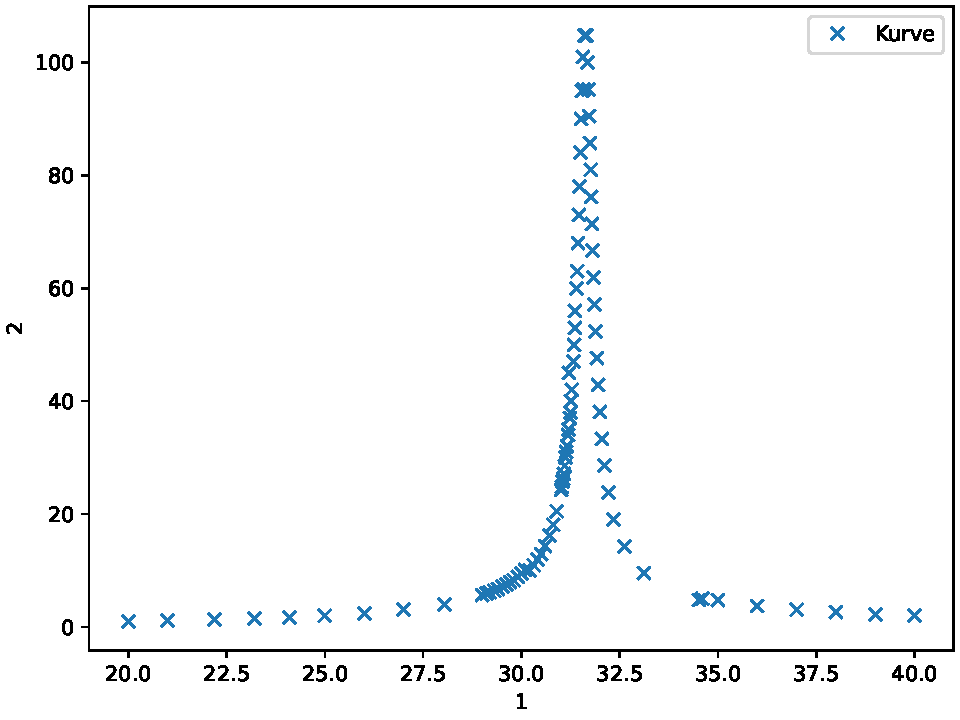
\includegraphics{plot.pdf}
%   \caption{Plot.}
%   \label{fig:plot}
% \end{figure}

%Siehe \autoref{fig:plot}!